%\iffalse
\let\negmedspace\undefined
\let\negthickspace\undefined
\documentclass[journal,12pt,twocolumn]{IEEEtran}
\usepackage{cite}
\usepackage{amsmath,amssymb,amsfonts,amsthm}
\usepackage{algorithmic}
\usepackage{graphicx}
\usepackage{textcomp}
\usepackage{xcolor}
\usepackage{txfonts}
\usepackage{listings}
\usepackage{enumitem}
\usepackage{mathtools}
\usepackage{gensymb}
\usepackage{comment}
\usepackage[breaklinks=true]{hyperref}
\usepackage{tkz-euclide} 
\usepackage{listings}
\usepackage{gvv}                                        
\def\inputGnumericTable{}                                 
\usepackage[latin1]{inputenc}                                
\usepackage{color}                                            
\usepackage{array}                                            
\usepackage{longtable}                                       
\usepackage{calc}                                             
\usepackage{multirow}                                         
\usepackage{hhline}                                           
\usepackage{ifthen}                                           
\usepackage{lscape}
\newtheorem{theorem}{Theorem}[section]
\newtheorem{problem}{Problem}
\newtheorem{proposition}{Proposition}[section]
\newtheorem{lemma}{Lemma}[section]
\newtheorem{corollary}[theorem]{Corollary}
\newtheorem{example}{Example}[section]
\newtheorem{definition}[problem]{Definition}
\newcommand{\BEQA}{\begin{eqnarray}}
\newcommand{\EEQA}{\end{eqnarray}}
\newcommand{\define}{\stackrel{\triangle}{=}}
\theoremstyle{remark}
\newtheorem{rem}{Remark}
\begin{document}

\bibliographystyle{IEEEtran}
\vspace{3cm}

\title{DISCRETE}
\author{EE23BTECH11006 - Ameen Aazam$^{*}$% <-this % stops a space
}
\maketitle
\newpage
\bigskip

\renewcommand{\thefigure}{\theenumi}
\renewcommand{\thetable}{\theenumi}

\vspace{3cm}
\textbf{Question :}
Find the sum of the following APs:
\begin{enumerate}[label=(\alph*)]
\item $2, 7, 12, \ldots$ to $10$ terms.
\item $-37, -33, -29, \ldots$ to $12$ terms.
\item $0.6, 1.7, 2.8, \ldots$ to $100$ terms.
\item $\frac{1}{15}, \frac{1}{12}, \frac{1}{10}, \ldots$ to $11$ terms.
\end{enumerate}
\solution
%\fi
\begin{table}[htbp]
    \centering
    \begin{tabular}{|c|c|c|} \hline
      \textbf{Input Parameters} & \textbf{Values} & \textbf{Description} \\ \hline
      $n$ & & Independent Variable \\ \hline
      $a$ & & First term of $1^{st}$ G.P. \\ \hline
      $r$ & & Common ratio of $1^{st}$ G.P. \\ \hline
      $x_1\brak{n}$ & $x_1\brak{n}=ar^nu\brak{n}$& General term of $1^{st}$ G.P. \\ \hline
      $X_1\brak{z}$ & & z-Transform of $1^{st}$ G.P. \\ \hline
      $A$ & & First term of $2^{nd}$ G.P. \\ \hline
      $R$ & & Common ratio of $2^{nd}$ G.P. \\ \hline
      $x_2\brak{n}$ & $x_1\brak{n}=AR^nu\brak{n}$& General term of $2^{nd}$ G.P. \\ \hline
      $X_2\brak{z}$ & & z-Transform of $2^{nd}$ G.P. \\ \hline
    \end{tabular}
    \vspace{3pt}
    \caption{Parameters}
    \label{tab:11.9.3.20.tab}
\end{table}

We have the general terms,
\begin{align}
    x\brak{n}=\sbrak{x\brak{0}+nd}u\brak{n}
\end{align}
Now for sum,
\begin{align}
    &y\brak{n}=x\brak{n}\ast u\brak{n} \\
    &Y\brak{z}=X\brak{z}U\brak{z}
\end{align}
From \eqref{eq:abc}, we get $Y\brak{z}$ as,
\begin{align}
    Y\brak{z}=\frac{x\brak{0}}{\brak{1-z^{-1}}^2}+\frac{dz^{-1}}{\brak{1-z^{-1}}^3}
\end{align}
Now using contour integration for each case,
\begin{enumerate}[label=(\alph*)]
    \item \begin{align}
        &x\brak{0}=2 \\
        &d=5 \\
        &y\brak{n}=\frac{1}{2\pi j}\oint_{C}S\brak{z}z^{n-1}dz  \\
        &y\brak{n}=\frac{1}{2\pi j}\oint_{C}\brak{\dfrac{2z^{n-1}}{\brak{1-z^{-1}}^2} + \dfrac{5z^{n-2}}{\brak{1-z^{-1}}^{3}}}dz \\
    \end{align}
    For $R_1$ we can observe that the pole has been repeated twice.
\begin{align}
    R_1&=\frac{1}{\brak {1}!}\lim\limits_{z\to 1}\frac{d}{dz}\brak {{\brak{z-1}}^{2}\frac{2z^{n+1}}{{\brak{z-1}}^2}}\\
    &=2\brak{n+1}\lim\limits_{z\to 1}\brak{z^n}\\
    &=2\brak{n+1}\label{eq:a}
\end{align}
    For $R_2$ we can observe that the pole has been repeated thrice.
\begin{align}
    R_2&=\frac{1}{\brak {2}!}\lim\limits_{z\to 1}\frac{d^{2}}{dz^{2}}\brak {{\brak{z-1}}^{3}\frac{5z^{n+1}}{{\brak{z-1}}^3}}\\
    &=\frac{5\brak{n+1}}{2}\lim\limits_{z\to 1}\frac{d}{dz}\brak{z^n}\\
    &=\frac{5\brak{n+1}\brak{n}}{2}\lim\limits_{z\to 1}\brak{z^{n-1}}\\
    &=\frac{5\brak{n}\brak{n+1}}{2}\label{eq:b} \\
    \implies R&= R_1 + R_2
\end{align}
Using \eqref{eq:a} and \eqref{eq:b},
\begin{align}
   R &=2\brak{n+1}+\frac{5\brak{n}\brak{n+1}}{2}
\end{align}
Finally,
\begin{align}
    y\brak{n}&=2\brak{n+1}u\brak{n}+5\brak{\dfrac{{n\brak{n+1}}}{2}}u\brak{n}\\
    &=\dfrac{n+1}{2}\brak{4+5n}u\brak{n} \\
    y\brak{9}&=245
\end{align}
    \begin{figure}[h!]
        \centering
        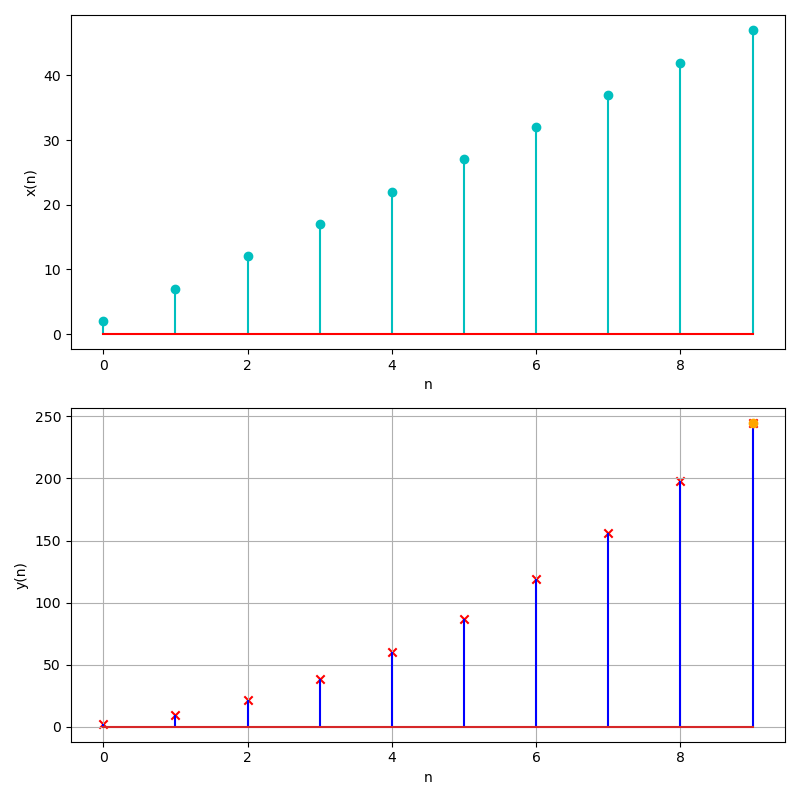
\includegraphics[width=\columnwidth]{figs/plt1.png}
        \caption{$1st$ AP}
    \end{figure}
    \item \begin{align}
        &x\brak{0}=-37 \\
        &d=4 \\
        &y\brak{n}=\frac{1}{2\pi j}\oint_{C}\brak{\dfrac{-37z^{n-1}}{\brak{1-z^{-1}}^2} + \dfrac{4z^{n-2}}{\brak{1-z^{-1}}^{3}}}dz \\
    \end{align}
    For $R_1$ the pole has been repeated twice.
\begin{align}
    R_1&=\frac{1}{\brak {1}!}\lim\limits_{z\to 1}\frac{d}{dz}\brak {{\brak{z-1}}^{2}\frac{-37z^{n+1}}{{\brak{z-1}}^2}}\\
    &=-37\brak{n+1}\lim\limits_{z\to 1}\brak{z^n}\\
    &=-37\brak{n+1}\label{eq:c}
\end{align}
    For $R_2$ the pole has been repeated thrice.
\begin{align}
    R_2&=\frac{1}{\brak {2}!}\lim\limits_{z\to 1}\frac{d^{2}}{dz^{2}}\brak {{\brak{z-1}}^{3}\frac{4z^{n+1}}{{\brak{z-1}}^3}}\\
    &=\frac{4\brak{n+1}}{2}\lim\limits_{z\to 1}\frac{d}{dz}\brak{z^n}\\
    &=\frac{4\brak{n+1}\brak{n}}{2}\lim\limits_{z\to 1}\brak{z^{n-1}}\\
    &=\frac{4\brak{n}\brak{n+1}}{2}\label{eq:d}
\end{align}
Using \eqref{eq:c} and \eqref{eq:d},
\begin{align}
    &y\brak{n}=\dfrac{n+1}{2}\brak{-74+4n}u\brak{n}\\
    &y\brak{11}=-180
\end{align}
    \begin{figure}[h!]
        \centering
        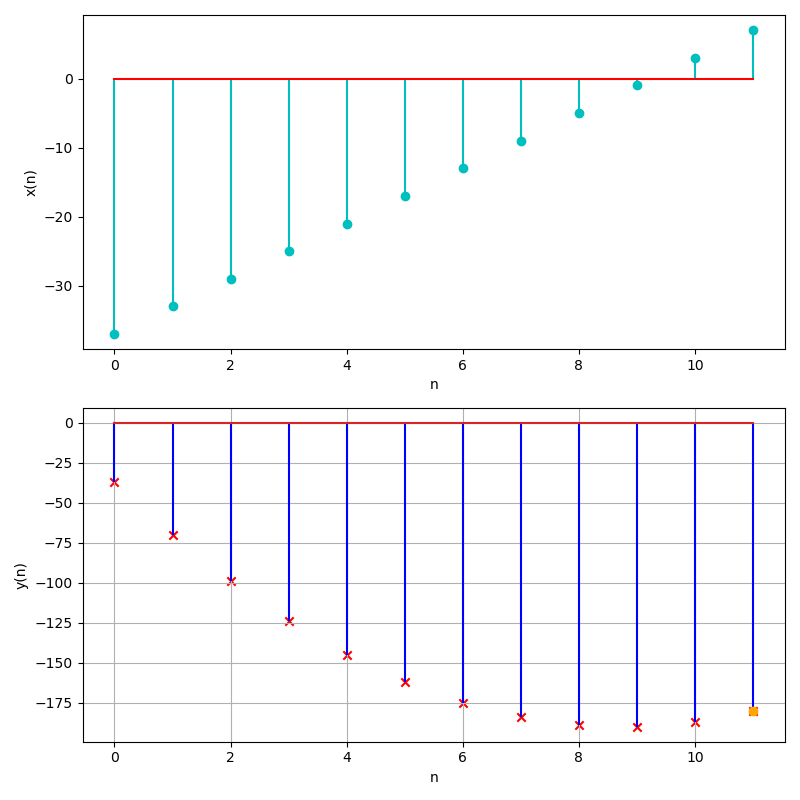
\includegraphics[width=\columnwidth]{figs/plt2.png}
        \caption{$2nd$ AP}
    \end{figure}
    \\item \begin{align}
        &x\brak{0}=0.6 \\
        &d=1.1 \\
        &y\brak{n}=\frac{1}{2\pi j}\oint_{C}\brak{\dfrac{0.6z^{n-1}}{\brak{1-z^{-1}}^2} + \dfrac{1.1z^{n-2}}{\brak{1-z^{-1}}^{3}}}dz \\
    \end{align}
    For $R_1$ the pole is repeated twice.
\begin{align}
    R_1&=\frac{1}{\brak {1}!}\lim\limits_{z\to 1}\frac{d}{dz}\brak {{\brak{z-1}}^{2}\frac{0.6z^{n+1}}{{\brak{z-1}}^2}}\\
    &=0.6\brak{n+1}\lim\limits_{z\to 1}\brak{z^n}\\
    &=0.6\brak{n+1}\label{eq:e}
\end{align}
    For $R_2$ the pole is repeated thrice.
\begin{align}
    R_2&=\frac{1}{\brak {2}!}\lim\limits_{z\to 1}\frac{d^{2}}{dz^{2}}\brak {{\brak{z-1}}^{3}\frac{1.1z^{n+1}}{{\brak{z-1}}^3}}\\
    &=\frac{1.1\brak{n+1}}{2}\lim\limits_{z\to 1}\frac{d}{dz}\brak{z^n}\\
    &=\frac{1.1\brak{n+1}\brak{n}}{2}\lim\limits_{z\to 1}\brak{z^{n-1}}\\
    &=\frac{1.1\brak{n}\brak{n+1}}{2}\label{eq:f}
\end{align}
Using \eqref{eq:e} and \eqref{eq:f},
\begin{align}
    &y\brak{n}=\dfrac{n+1}{2}\brak{1.2+1.1n}u\brak{n}\\
    &y\brak{99}=5505
\end{align}
    \begin{figure}[h!]
        \centering
        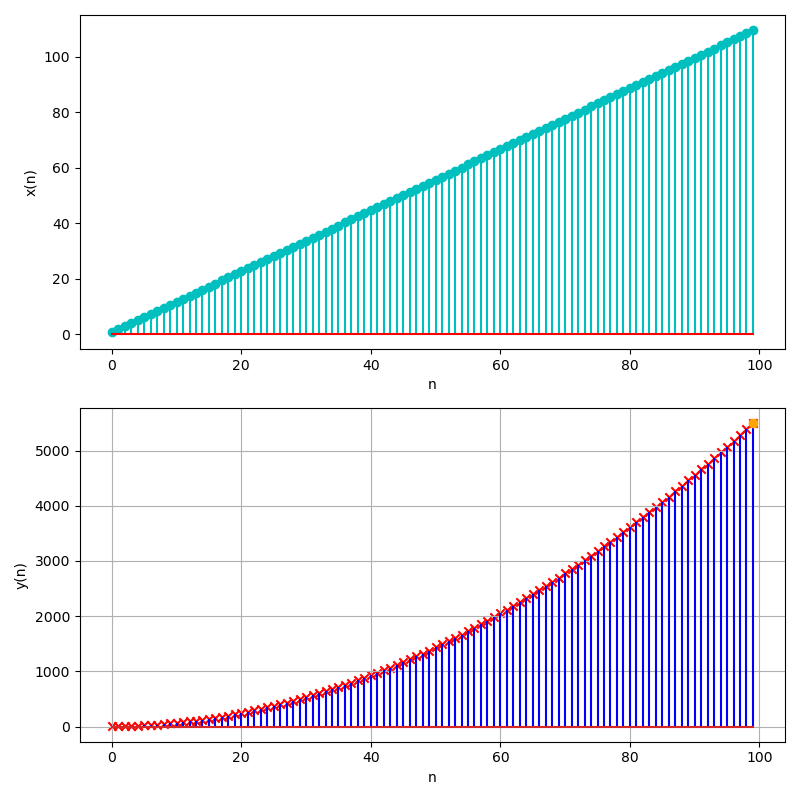
\includegraphics[width=\columnwidth]{figs/plt3.png}
        \caption{$4th$ AP}
    \end{figure}

\item \begin{align}
        &x\brak{0}=\frac{1}{15} \\
        &d=\frac{1}{60} \\
        &y\brak{n}=\frac{1}{2\pi j}\oint_{C}\brak{\dfrac{\frac{1}{15}z^{n-1}}{\brak{1-z^{-1}}^2} + \dfrac{1.1z^{n-2}}{\brak{1-z^{-1}}^{3}}}dz \\
    \end{align}
    For $R_1$ the pole is repeated twice.
\begin{align}
    R_1&=\frac{1}{\brak {1}!}\lim\limits_{z\to 1}\frac{d}{dz}\brak {{\brak{z-1}}^{2}\frac{\frac{1}{15}z^{n+1}}{{\brak{z-1}}^2}}\\
    &=\frac{1}{15}\brak{n+1}\lim\limits_{z\to 1}\brak{z^n}\\
    &=\frac{1}{15}\brak{n+1}\label{eq:g}
\end{align}
    For $R_2$ the pole is repeated thrice.
\begin{align}
    R_2&=\frac{1}{\brak {2}!}\lim\limits_{z\to 1}\frac{d^{2}}{dz^{2}}\brak {{\brak{z-1}}^{3}\frac{\frac{1}{60}z^{n+1}}{{\brak{z-1}}^3}}\\
    &=\frac{\frac{1}{60}\brak{n+1}}{2}\lim\limits_{z\to 1}\frac{d}{dz}\brak{z^n}\\
    &=\frac{\frac{1}{60}\brak{n+1}\brak{n}}{2}\lim\limits_{z\to 1}\brak{z^{n-1}}\\
    &=\frac{\frac{1}{60}\brak{n}\brak{n+1}}{2}\label{eq:h}
\end{align}
Using \eqref{eq:g} and \eqref{eq:h},
\begin{align}
    &y\brak{n}=\dfrac{n+1}{2}\brak{\frac{2}{15}+\frac{n}{60}}u\brak{n}\\
    &y\brak{10}=1.65
\end{align}
\begin{figure}[h!]
        \centering
        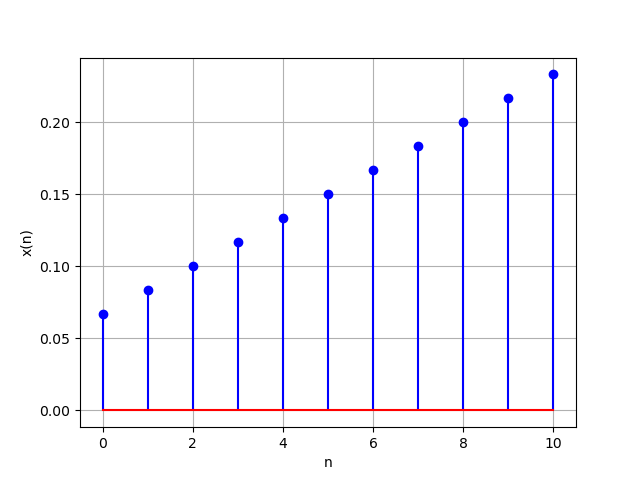
\includegraphics[width=\columnwidth]{figs/plt4.png}
        \caption{$4th$ AP}
    \end{figure}
\end{enumerate}

\end{document}

